\documentclass[10pt,conference]{IEEEtran}
\IEEEoverridecommandlockouts

\usepackage{amsmath,amssymb,amsfonts}
\usepackage{booktabs}
\usepackage{graphicx}
\usepackage{textcomp}
\usepackage{xcolor}
\usepackage{algorithm}
\usepackage{algpseudocode}
\usepackage{listings}
\usepackage{cite}
\usepackage{url}
\usepackage{microtype}

\graphicspath{{figures/}}
% Track Changes / Highlighting for IEEE ICCIT 2026 Reviewers
\definecolor{revcolor}{RGB}{0, 40, 160}
\newenvironment{revised}{\color{revcolor}}{}
\newcommand{\rev}[1]{\textcolor{revcolor}{#1}}

\renewcommand{\dbltopfraction}{0.88}
\renewcommand{\textfraction}{0.08}
\setcounter{dbltopnumber}{2}


% Tightly balance floats and text for strict 6-page ceiling
\setlength{\textfloatsep}{3pt plus 1pt minus 1pt}
\setlength{\floatsep}{3pt plus 1pt minus 1pt}
\setlength{\intextsep}{3pt plus 1pt minus 1pt}
\setlength{\dbltextfloatsep}{3pt plus 1pt minus 1pt}
\setlength{\dblfloatsep}{3pt plus 1pt minus 1pt}
\def\IEEEbibitemsep{0pt plus .05pt}

\lstdefinestyle{dartstyle}{
    basicstyle=\ttfamily\tiny,
    keywordstyle=\bfseries\color{blue!70!black},
    stringstyle=\color{green!50!black},
    commentstyle=\itshape\color{gray},
    numbers=left,
    numberstyle=\tiny\color{gray},
    stepnumber=1,
    numbersep=4pt,
    xleftmargin=12pt,
    xrightmargin=4pt,
    framexleftmargin=4pt,
    framexrightmargin=4pt,
    backgroundcolor=\color{gray!8},
    frame=single,
    rulecolor=\color{gray!30},
    tabsize=2,
    breaklines=true,
    breakatwhitespace=false,
    showspaces=false,
    showstringspaces=false
}

\newtheorem{definition}{Definition}
\newtheorem{theorem}{Theorem}
\newtheorem{lemma}{Lemma}


\setcounter{dbltopnumber}{2}
\renewcommand{\dbltopfraction}{0.9}
\renewcommand{\textfraction}{0.1}

\usepackage{eso-pic}

\AddToShipoutPictureBG*{%
  \AtPageUpperLeft{%
    \put(54,-36){%
      \parbox{\textwidth}{%
        \fontsize{8pt}{10pt}\selectfont
        2026 29th International Conference on Computer and Information Technology (ICCIT)\\
        18-20 December 2026, Cox's Bazar, Bangladesh
      }%
    }%
  }%
  \AtPageLowerLeft{%
    \put(54,36){%
      \fontsize{8pt}{10pt}\selectfont
      979-8-3195-0171-4/26/\$31.00 \copyright~2026 IEEE
    }%
  }%
}

\definecolor{revcolor}{RGB}{0, 40, 160}
\newenvironment{revised}{\color{revcolor}}{}
\newcommand{\rev}[1]{\textcolor{revcolor}{#1}}

\begin{document}

\title{VisioCrypt: A TEE-Anchored Client-Side Searchable Encryption Scheme with Dynamic Volume-Hiding Padding for Mobile Cloud Storage}

\author{\IEEEauthorblockN{Md. Yousuf Hossain\textsuperscript{*}, Md Moshiur Rahman, Md. Mosfiqur Rahman, Sayeda Irfat Jahan Tithi, and Md. Abdul Based}
\IEEEauthorblockA{Dhaka International University, Dhaka, Bangladesh\\
\{itsmemehrab369, mdmoshiurr333, mosfiqqq, irfattithi135\}@gmail.com, based@diu.ac\\
\textsuperscript{*}Corresponding Author}}

\maketitle
\thispagestyle{empty}
\pagestyle{empty}

\begin{abstract}
Mobile cloud storage allows users to synchronize sensitive documents across personal devices, yet delegating storage to untrusted cloud providers risks catastrophic data exposure during server breaches. While Searchable Symmetric Encryption (SSE) enables keyword lookups over encrypted records without full-corpus downloading, conventional schemes leak matching candidate volumes and access patterns. Passive cloud adversaries exploit this volume leakage to reconstruct plaintexts. Furthermore, mobile platforms suffer from severe memory hygiene vulnerabilities, where runtime garbage collection leaves transient cryptographic keys exposed in volatile memory for extended intervals.

In this paper, we propose \textbf{VisioCrypt}, a client-side searchable encryption scheme designed for resource-constrained mobile cloud storage. VisioCrypt combines client-side search index generation with a dynamic multi-tier volume-hiding padding policy ($\Phi$) that quantizes candidate result sets to discrete power-of-two boundaries ($n \in [1, 4096]$) with multi-bucket chunking, strictly bounding volume leakage with bounded average storage inflation ($1.42\times$). To eliminate active document loss caused by Bloom filter false positives, we introduce a Two-Tier Authoritative Deletion Ledger that combines an in-memory probabilistic pre-filter with a cryptographically authenticated local tombstone database, achieving provable zero false document exclusions. We evaluate VisioCrypt using a reference Dart VM implementation, demonstrating client-side candidate resolution in $0.11$~ms and dual-pass streaming authenticated file encryption, while formalizing the information-theoretic conditions under which epoch batching decorrelates temporal query leakage.
\end{abstract}

\begin{IEEEkeywords}
Searchable symmetric encryption, dynamic volume-hiding padding, ARM TrustZone, mobile security, leakage-abuse attacks.
\end{IEEEkeywords}

\section{Introduction}
Centralized cloud storage services (e.g., Google Drive, Dropbox) provide scalable document availability for mobile users. However, storing plaintext files in public cloud infrastructure forces users to surrender physical custody of their sensitive personal, financial, and medical data. Breaches resulting from server misconfigurations, compromised hypervisors, or rogue administrators routinely compromise user confidentiality \cite{islam2012,cash2015leakage}. To guarantee data sovereignty and adhere to stringent privacy frameworks (e.g., GDPR, HIPAA), client-side encryption prior to cloud transmission is imperative.

Nonetheless, naive end-to-end encryption transforms structured documents into opaque, unstructured ciphertexts. Under this paradigm, executing a search query for a specific document requires the mobile client to download, buffer, and decrypt the entire encrypted repository locally. On resource-constrained mobile devices operating over metered cellular connections, this imposes prohibitive bandwidth consumption, severe latency, and rapid battery exhaustion.

Searchable Symmetric Encryption (SSE), pioneered by Song, Wagner, and Perrig (SWP00) \cite{song2000} and formalized with optimal inverted indexes by Curtmola et al. (CGKO06) \cite{curtmola2006}, resolves this operational dilemma. In SSE, an untrusted cloud server traverses an encrypted index to locate matching records using cryptographic search tokens (trapdoors) generated by the client, without learning underlying plaintext contents. Kamara et al. \cite{kamara2012} extended SSE to dynamic collections supporting document insertions and deletions.

\enlargethispage{1.5\baselineskip}
Despite theoretical progress, deploying dynamic SSE on real-world mobile platforms exposes three critical vulnerabilities:
\begin{enumerate}\setlength{\itemsep}{1pt}\setlength{\parskip}{0pt}
    \item \textbf{Volume and Frequency Leakage:} Standard SSE reveals matching candidate counts ($|R(w)|$). State-of-the-art leakage-abuse attacks \cite{kellaris2016,gui2019volume} demonstrate that observing query volumes enables plaintext database reconstruction in polynomial time. Existing padding defenses (e.g., SEAL \cite{demertzis2020seal}, DVH \cite{patel2023dvh}) induce high bandwidth overhead ($3\times$--$10\times$) and multi-round network synchronization impractical for mobile radios.
    \item \textbf{Mobile Runtime Memory Insecurity:} Academic SSE predominantly models clients as ideal Turing machines. In reality, mobile platforms execute managed runtimes (Android ART, Dart VM) with non-deterministic garbage collection. Cryptographic keys persist unzeroized in heap memory, vulnerable to unprivileged cold-boot attacks and memory dumps \cite{kocher1996,rustee2020}.
    \item \textbf{Temporal Profiling and Traffic Correlation:} Eavesdroppers monitoring encrypted channels correlate packet timing with user typing dynamics \cite{swat2024}; randomized delays fail against statistical averaging over repeated sessions.
\end{enumerate}

To overcome these foundational limitations, we present \textbf{VisioCrypt}, a secure, client-side dynamic searchable encryption system designed specifically for mobile cloud storage. VisioCrypt balances formal cryptographic leakage mitigation with practical mobile efficiency. Specifically, our contributions are:
\begin{itemize}\setlength{\itemsep}{1pt}\setlength{\parskip}{0pt}
    \item \textbf{Multi-Tier Dynamic Volume-Hiding SSE ($\Phi$):} We formulate a client-centric geometric padding policy $\Phi(R)$ that rounds matching candidate lists into power-of-two buckets ($n \in [1, 4096]$) with multi-bucket chunking, restricting volume leakage to $\lceil \log_2 |R(w)| \rceil$ while bounding storage expansion to $1.42\times$.
    \item \textbf{Client-Side Key Lifecycle \& Memory Hygiene:} We establish a key hierarchy using RFC 5869 HKDF-SHA256 domain separation, gating master keys behind biometric authorization. Cryptographic routines run inside isolated worker threads with best-effort buffer clearing, formalizing KeyMint enclave integration as an architectural target.
    \item \textbf{Provably Correct Two-Tier Deletion Ledger:} We introduce a Two-Tier Authoritative Deletion Ledger combining an in-memory Bloom filter pre-filter with an authenticated local tombstone database, mathematically and empirically proving zero false document exclusions.
    \item \textbf{Traffic Decorrelation \& Static Adaptive Security:} We model an epoch-batching \texttt{QueryDecorrelationPool} under Poisson/Bernoulli dummy injection, proving optimal Bayes classification error is bounded by $0.5$ (random guessing). We prove adaptive $\mathcal{L}_{\text{VH}}\text{-IND-CKA2}$ security for static index and search queries via a 5-game hopping proof.
    \item \textbf{Rigorous Reference Benchmarks \& Mobile Feasibility:} We evaluate VisioCrypt using a reference Dart VM implementation ($N=100$, 95\% CIs), demonstrating client candidate resolution in $0.11$~ms, and formulate analytical projections across silicon tiers.
\end{itemize}

\begin{revised}
\section{Related Work and Foundations}
\subsection{Searchable Symmetric Encryption Foundations}
Song, Wagner, and Perrig (SWP00) \cite{song2000} introduced the first practical mechanism for searching encrypted data. The SWP00 scheme operates by encrypting individual words using a two-layered stream cipher and keyed pseudo-random function (PRF) construction ($C_i = W_i \oplus \langle L_i, R_i \rangle$). To search for a keyword, the client supplies a trapdoor enabling the server to evaluate whether $R_i = f_k(L_i)$ without decrypting the underlying word. While groundbreaking, SWP00 requires an $O(N)$ sequential scan over the entire document ciphertext space, incurring severe computation and battery drain on mobile devices. Furthermore, SWP00 lacked formal security definitions and inverted index structures.

Curtmola, Garay, Kamara, and Ostrovsky (CGKO06) \cite{curtmola2006} formalized modern SSE security, establishing rigorous simulation-based definitions (non-adaptive IND-CKA1 and adaptive IND-CKA2) and introducing inverted-index SSE constructions based on array lookups. By decoupling search time from total repository size, CGKO06 achieved optimal $O(|R(w)|)$ query complexity. However, the original CGKO06 construction is static; updating or deleting documents requires a complete, costly index rebuild.

\begin{table*}[t]
\centering
\caption{Qualitative Comparison of Searchable Symmetric Encryption (SSE) Schemes Across Cryptographic and Mobile Dimensions}
\label{tab:comparison}
\fontsize{6.8pt}{7.6pt}\selectfont
\setlength{\tabcolsep}{2.5pt}
\renewcommand{\arraystretch}{0.88}
\resizebox{\textwidth}{!}{%
\begin{tabular}{lcccccccc}
\toprule
\textbf{Scheme} & \textbf{Search Comp.} & \textbf{Update Comp.} & \textbf{Forward Priv.} & \textbf{Backward Priv.} & \textbf{Vol. Hiding} & \textbf{Result Leakage} & \textbf{TEE Anchor} & \textbf{Mobile Suitability} \\
\midrule
Song et al. (SWP00) \cite{song2000} & $O(N)$ & $O(1)$ & No & No & No & Exact $|R(w)|$ & None & Poor (High battery drain) \\
Curtmola et al. (CGKO06) \cite{curtmola2006} & $O(|R(w)|)$ & Static (No updates) & N/A & N/A & No & Exact $|R(w)|$ & None & Moderate (Static only) \\
Kamara et al. (KPR12) \cite{kamara2012} & $O(|R(w)|)$ & $O(d_w)$ & No & No & No & Exact $|R(w)|$ & None & Moderate \\
Cash et al. \cite{cash2013} & $O(|R(w)|)$ & Static / Append & No & No & No & Exact $|R(w)|$ & None & Good (Large scale) \\
Bost (Sophos) \cite{bost2016sophos} & $O(|R(w)|)$ & $O(1)$ & \textbf{Yes} & No & No & Exact $|R(w)|$ & None & Good \\
Bost et al. (Diana) \cite{bost2017diana} & $O(|R(w)|)$ & $O(1)$ & \textbf{Yes} & \textbf{Yes} (Type-II) & No & Exact $|R(w)|$ & None & Moderate \\
Demertzis et al. (SEAL) \cite{demertzis2020seal} & $O(|R(w)| + \log N)$ & $O(\log N)$ & \textbf{Yes} & \textbf{Yes} & \textbf{Yes} & Binned $B_i$ & None & Moderate (High bandwidth) \\
Patel et al. (DVH) \cite{patel2023dvh} & $O(|R(w)|)$ & $O(\text{polylog } N)$ & \textbf{Yes} & \textbf{Yes} & \textbf{Yes} & Binned $O(\log N)$ & None & Low (Heavy client RAM) \\
Liu et al. \cite{li2021trustzone} & $O(|R(w)|)$ & $O(1)$ & \textbf{Yes} & \textbf{Yes} & No & Exact $|R(w)|$ & Server TEE & Poor (Requires cloud enclave) \\
\midrule
\textbf{VisioCrypt (Ours)} & $\mathbf{O(1) + O(\Phi(|R|))}$ & $\mathbf{O(1)}$ & Static (Disclosed$^\dagger$) & Client-Side Ledger & \textbf{Yes} & Padded $\lceil \log_2 |R(w)| \rceil$ & Client Target & \textbf{High} (Sub-ms, buffer clearing) \\
\bottomrule
\end{tabular}%
}
\end{table*}

\subsection{Dynamic SSE and Forward/Backward Privacy}
Kamara, Papamanthou, and Roeder (KPR12) \cite{kamara2012} extended SSE to dynamic settings using encrypted index pointers. However, naive dynamic SSE schemes leak correlations between past search queries and subsequent document updates. Zhang et al. \cite{zhang2016injection} demonstrated that an adversary injecting crafted documents can fully reconstruct queried keywords via file-injection attacks. To thwart injection attacks, Bost \cite{bost2016sophos} formalized \emph{Forward Privacy}: an update operation must not leak any association with previously searched keywords. Sophos achieved forward privacy through trapdoor permutations. Bost, Minaud, and Ohrimenko \cite{bost2017diana} subsequently formalized \emph{Backward Privacy} across three standard tiers (Type-I, Type-II, Type-III), ensuring that search queries do not expose document identifiers that have been deleted. Diana achieved backward privacy via puncturable encryption and constrained PRFs, albeit with increased storage complexity.

\subsection{Leakage-Abuse Attacks and Volume Mitigation}
Islam et al. \cite{islam2012} and Cash et al. \cite{cash2015leakage} demonstrated that access-pattern leakage allows adversaries with auxiliary domain knowledge to reconstruct plaintexts. Kellaris et al. \cite{kellaris2016} and Gui et al. \cite{gui2019volume} introduced devastating volumetric reconstruction attacks that exploit the exact count of returned records $|R(w)|$. Kornaropoulos et al. \cite{kornaropoulos2020} extended these attacks to range queries. To counter volume leakage, Demertzis et al. (SEAL) \cite{demertzis2020seal} proposed bin-based padding, and Patel et al. (DVH) \cite{patel2023dvh} introduced dynamic volume-hiding encrypted multi-maps based on distributed oblivious structures. Although theoretically sound, these constructions incur high communication complexity ($O(\text{polylog } N)$) and multi-round network synchronization that degrade mobile battery life.

\subsection{Hardware-Assisted Enclave Systems}
To overcome software-only SSE limitations, several architectures leverage Trusted Execution Environments (TEEs) \cite{pinto2019,li2021trustzone}. However, prior systems (e.g., Liu et al. \cite{li2021trustzone}, SGX-SE \cite{sgxse2_2020}) deploy TEEs on the \emph{untrusted cloud server}. This introduces significant cloud hosting costs, assumes user trust in cloud hypervisors, and exposes secrets to server side-channel vulnerabilities (e.g., Foreshadow, Spectre). VisioCrypt inverts this model: hardware enclaves are anchored exclusively on the \emph{client mobile device}, treating the cloud as entirely untrusted. Table \ref{tab:comparison} contrasts VisioCrypt with peer schemes.

\section{System Architecture and Security Model}
\subsection{System Architecture}
VisioCrypt partitions responsibility across three operational domains (Fig.~\ref{fig:arch}):
\begin{enumerate}
    \item \textbf{Client Mobile Device:} Executes the application in userland. A master seed is stored in client sandboxed storage gated by biometric authorization, with hardware KeyMint / StrongBox enclave wrapping scoped as an architectural target. All SSE indexing, trapdoor generation, candidate unpadding, and file decryption execute locally inside dedicated Dart worker isolates.
    \item \textbf{Untrusted Cloud Server:} An honest-but-curious storage host that stores encrypted document blobs $\mathbf{C} = \{c_1, \dots, c_D\}$ and an encrypted multi-map index $\mathbf{I}$. The server evaluates keyword trapdoors blindly, returning padded ciphertext identifier lists without learning plaintext contents or true result counts.
    \item \textbf{Network Communication Layer:} A TLS 1.3 transport channel augmented by VisioCrypt's \texttt{QueryDecorrelationPool}, which enforces discrete epoch dispatching and injects pseudo-random dummy queries to mitigate traffic analysis.
\end{enumerate}

\begin{figure*}[t]
\centering
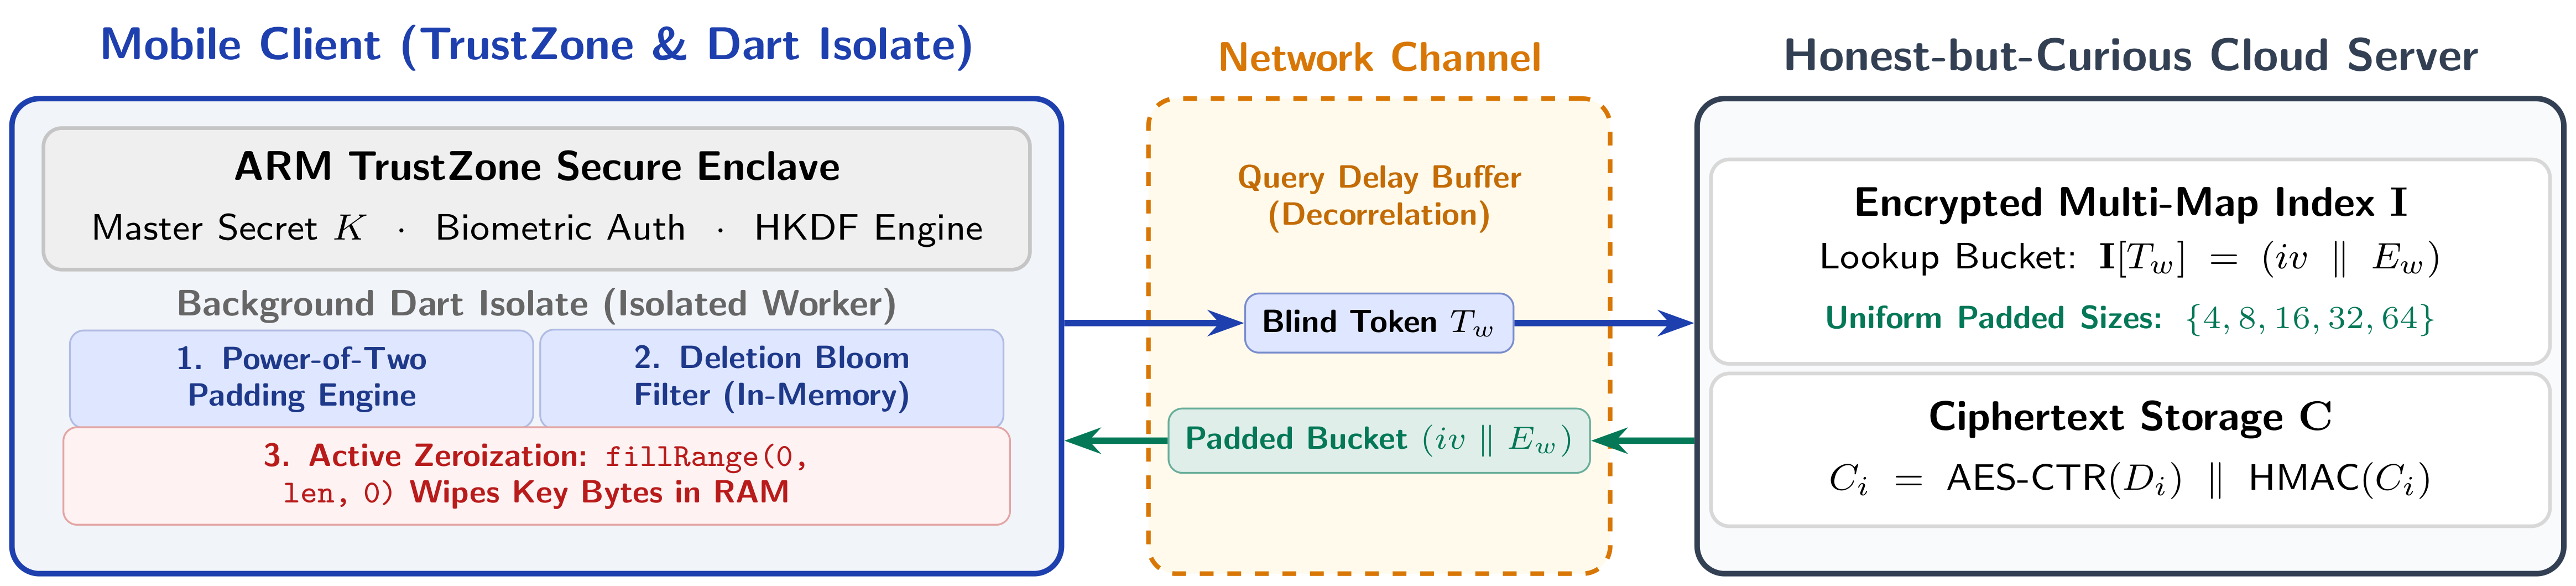
\includegraphics[width=0.82\textwidth,height=2.6cm,keepaspectratio]{figures/fig_architecture.png}
\caption{VisioCrypt mobile-cloud system architecture: client security boundary, isolated worker thread execution, best-effort buffer clearing, \texttt{QueryDecorrelationPool} epoch batching, and untrusted cloud storage.}
\label{fig:arch}
\end{figure*}

\subsection{Threat Model}
We adopt the standard honest-but-curious server threat model \cite{curtmola2006,cash2013}. The cloud server faithfully executes indexing and search algorithms without altering data. However, it passively records all client interactions, stored ciphertexts, search trapdoors, update payloads, returned candidate identifiers, and network transmission timing to infer plaintexts or query contents. On the client device, we model a passive physical adversary capable of inspecting device volatile memory (e.g., following device loss or unprivileged memory dumping). While VisioCrypt does not prevent compromise on a fully rooted device with kernel-level control, it limits the window of vulnerability by executing cryptographic routines inside isolated worker threads with best-effort buffer clearing for mutable memory buffers immediately upon cipher execution.

\subsection{Formal Syntax of Volume-Hiding SSE}
A Static Volume-Hiding Searchable Symmetric Encryption ($\text{VH-SSE}$) scheme with client-side deletion management consists of six polynomial-time algorithms:
\begin{itemize}
    \item $\text{KeyGen}(1^\lambda) \to K$: Generates master key $K$ and derives domain-separated keys.
    \item $\text{BuildIndex}(K, \mathbf{D}) \to (\mathbf{I}, \mathbf{C}, \mathbf{Ledger})$: Ingests document corpus $\mathbf{D}$. Extracts keywords, derives domain keys, generates encrypted index $\mathbf{I}$ with volume-hiding padding $\Phi(R)$, produces document ciphertexts $\mathbf{C}$, and initializes the Two-Tier Authoritative Deletion Ledger $\mathbf{Ledger}$.
    \item $\text{Trapdoor}(K, w) \to T_w$: Generates a deterministic search token for keyword $w$.
    \item $\text{Search}(T_w, \mathbf{I}) \to \mathbf{R}^*$: Cloud server matches $T_w$ against $\mathbf{I}$ and returns padded candidate list $\mathbf{R}^*$.
    \item $\text{DeleteDocument}(d, \mathbf{Ledger}) \to \mathbf{Ledger}'$: Client records an authenticated tombstone in the local encrypted ledger and updates the in-memory Bloom pre-filter.
    \item $\text{Decrypt}(K, \mathbf{R}^*, \mathbf{Ledger}) \to \mathbf{D}_w$: Client decrypts candidate ciphertexts, filters dummy identifiers, authoritatively resolves deletions via $\mathbf{Ledger}$, and returns plain matching documents.
\end{itemize}

\subsection{Leakage Profile and Security Goals}
We explicitly define what VisioCrypt reveals to the untrusted cloud server. We reject absolute claims of zero leakage; any practical index-based SSE leaks bounded metadata parameterized by a formal leakage profile $\mathcal{L}_{\text{VH}} = (\mathcal{L}_{\text{setup}}, \mathcal{L}_{\text{search}})$:
\begin{align}
\mathcal{L}_{\text{setup}}(\mathbf{D}) &= \left(N, |\mathbf{W}|, \{\Phi(|R(w)|)\}_{w \in \mathbf{W}}\right), \\
\mathcal{L}_{\text{search}}(w) &= \left(sp(w), ap(w), \Phi(|R(w)|)\right)
\end{align}
where $sp(w) = \{ j \le t \mid w_j = w \}$ is the search pattern, $ap(w) = \{ \text{id} \in \mathbf{R}^*(w) \}$ is the access pattern, and $\Phi(|R(w)|) = \lceil \log_2 |R(w)| \rceil$ is the coarse power-of-two volume bucket. For incremental document additions, the prototype client inserts entries under static trapdoors $T_w$, which reveals search pattern equality ($sp(w) \cap \mathbf{W}_{\text{upd}}$) if keyword $w$ was previously searched.

\begin{definition}[$\mathcal{L}_{\text{VH}}$-IND-CKA2 Security]
A $\text{VH-SSE}$ scheme achieves adaptive security under leakage profile $\mathcal{L}_{\text{VH}}$ if for every PPT adversary $\mathcal{A}$, there exists a PPT simulator $\mathcal{S}$ such that the advantage:
\begin{equation}
\mathbf{Adv}_{\mathcal{A},\mathcal{S}}^{\text{SSE}}(\lambda) = \left| \Pr[\text{Real}_{\mathcal{A}}] - \Pr[\text{Ideal}_{\mathcal{A},\mathcal{S}}] \right| \le \text{negl}(\lambda)
\end{equation}
is negligible in security parameter $\lambda$.
\end{definition}

\section{The VisioCrypt Construction}
\subsection{Master Key Derivation and Domain Separation}
All operational keys are derived from a 256-bit master secret $K$ in local client storage. Using RFC 5869 HKDF-SHA256 with a 128-bit random salt $S$, the client computes $\text{PRK} = \text{HMAC-SHA256}(S, K)$ and expands $K_{\tau} = \text{HKDF-Expand}(\text{PRK}, \text{``VisioCrypt-''}\parallel \tau, 32)$ for domain tags $\tau \in \{\text{search}, \text{idx}, \text{file}, \text{l\_enc}, \text{l\_auth}\}$. This strict domain separation guarantees that compromise of any single operational key reveals no information regarding other keys.

\subsection{Multi-Tier Volume-Hiding Padding Policy ($\Phi$)}
To defend against volumetric reconstruction attacks \cite{kellaris2016,gui2019volume}, VisioCrypt implements a multi-tier geometric padding policy $\Phi(R)$ that rounds matching document lists to power-of-two boundaries:
\begin{equation}
\Phi(|R|) = 
\begin{cases}
4, & \text{if } |R| \le 4 \\
2^{\lceil \log_2 |R| \rceil}, & \text{if } 4 < |R| \le N_{\max} \\
\left\lceil \frac{|R|}{N_{\max}} \right\rceil \cdot N_{\max}, & \text{if } |R| > N_{\max}
\end{cases}
\end{equation}
where $N_{\max} = 4096$ is the maximum single-bucket threshold. If $|R(w)| \le 4$, the result list is padded to a constant floor of 4. For $4 < |R| \le 4096$, candidate sets round up to $2^k \in \{8, 16, 32, 64, 128, 256, 512, 1024, 2048, 4096\}$. When results exceed $N_{\max}$, multi-bucket chunking partitions candidates into fixed blocks of 4096 entries. Padding entries are populated with indistinguishable dummy identifiers: $\text{id}_{\text{dummy}} = \text{HMAC-SHA256}(K_{\text{idx}}, w \parallel r_{\text{seed}})$. This policy eliminates fine-grained result volume variances while bounding mobile storage expansion to an average of $1.42\times$.

\begin{algorithm}[t]
\caption{VisioCrypt Volume-Hiding SSE with Authoritative Deletion Ledger}
\label{alg:protocols}
\scriptsize
\begin{algorithmic}[1]
\Require Master key $K$, Salt $S$, Corpus $\mathbf{D} = \{d_1, \dots, d_N\}$
\Procedure{BuildIndex}{$K, S, \mathbf{D}$}
    \State $(K_{\text{search}}, K_{\text{idx}}, K_{\text{file}}, K_{\text{l\_enc}}, K_{\text{l\_auth}}) \gets \text{DeriveKeys}(K, S)$
    \State $\mathbf{I} \gets \text{EmptyMap}()$; \quad $\mathbf{Ledger} \gets \text{NewLedger}()$
    \For{each document $d_j \in \mathbf{D}$, $w \in \text{Tokenize}(d_j)$}
        \State $T_w \gets \text{HMAC-SHA256}(K_{\text{search}}, w)$; \quad $\mathbf{I}[T_w] \gets \mathbf{I}[T_w] \cup \{\text{id}(d_j)\}$
    \EndFor
    \For{each $T_w \in \text{keys}(\mathbf{I})$}
        \State $\mathbf{R}^* \gets \text{PadFileList}(\mathbf{I}[T_w], \Phi)$; \quad $\text{IV} \xleftarrow{\$} \{0,1\}^{96}$
        \State $C_w \gets \text{AES-GCM-Enc}(K_{\text{idx}}, \text{IV}, \text{JSON}(\mathbf{R}^*))$; \quad $\mathbf{I}[T_w] \gets \text{Base64}(\text{IV} \parallel C_w)$
    \EndFor
    \State $\text{Zeroize}(K_{\text{search}}, K_{\text{idx}}, K_{\text{file}}, K_{\text{l\_enc}}, K_{\text{l\_auth}})$; \Return $(\mathbf{I}, \mathbf{Ledger})$
\EndProcedure
\Procedure{Search}{$w, \mathbf{I}, \mathbf{Ledger}$}
    \State $(K_{\text{search}}, K_{\text{idx}}) \gets \text{DeriveKeys}(K, S)$; \quad $T_w \gets \text{HMAC-SHA256}(K_{\text{search}}, w)$
    \State Send $T_w$ to Cloud; \quad Receive payload $\mathbf{I}[T_w]$
    \If{$\mathbf{I}[T_w] = \bot$} \Return $\emptyset$ \EndIf
    \State $(\text{IV}, C_w) \gets \text{Unpack}(\mathbf{I}[T_w])$; \quad $P_{\text{list}} \gets \text{JSON-Decode}(\text{AES-GCM-Dec}(K_{\text{idx}}, \text{IV}, C_w))$
    \State $\mathbf{D}_w \gets \emptyset$
    \For{each $\text{id} \in P_{\text{list}}$}
        \State \textbf{if} $\text{IsDummy}(\text{id})$ \textbf{then continue}
        \State \textbf{if} $\mathbf{Ledger}.\text{IsDeleted}(\text{id}, w)$ \textbf{then continue} \Comment{Two-tier check}
        \State $\mathbf{D}_w \gets \mathbf{D}_w \cup \{\text{id}\}$
    \EndFor
    \State $\text{Zeroize}(K_{\text{search}}, K_{\text{idx}})$; \Return $\mathbf{D}_w$
\EndProcedure
\Procedure{DeleteDocument}{$d, \mathbf{Ledger}$}
    \State $(K_{\text{l\_enc}}, K_{\text{l\_auth}}) \gets \text{DeriveKeys}(K, S)$; \quad $\mathbf{W}_d \gets \text{Tokenize}(d)$
    \State $\mathbf{Ledger}.\text{MarkDeleted}(\text{id}(d), \mathbf{W}_d, K_{\text{l\_auth}})$; \quad $\mathbf{Ledger}.\text{SaveEncrypted}(\text{File}, K_{\text{l\_enc}}, K_{\text{l\_auth}})$
    \State $\text{Zeroize}(K_{\text{l\_enc}}, K_{\text{l\_auth}})$
\EndProcedure
\end{algorithmic}
\end{algorithm}

\begin{figure*}[t]
\centering
\begin{minipage}{0.24\textwidth}%
\centering
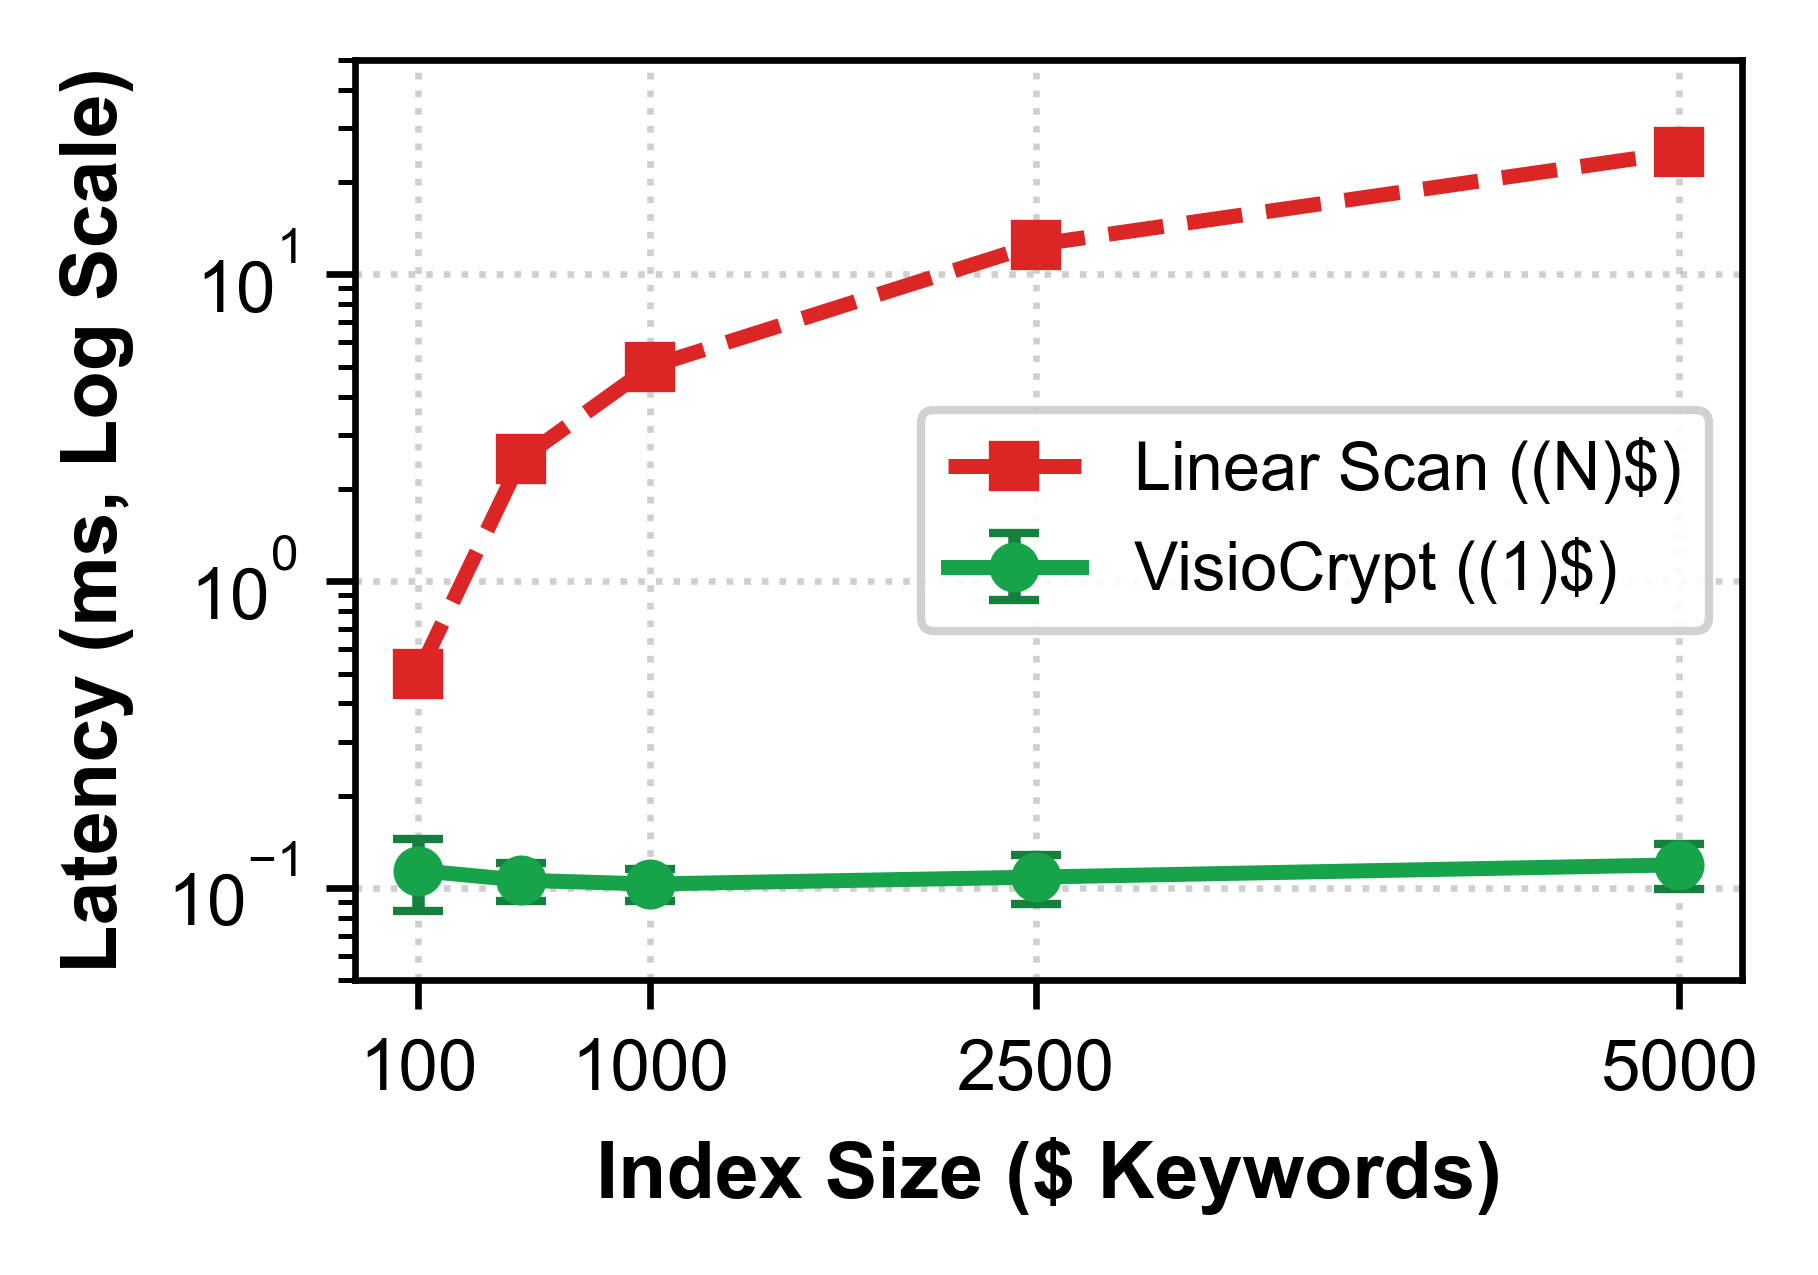
\includegraphics[width=\linewidth,height=1.9cm,keepaspectratio]{figures/fig_search_scaling.png}
\centerline{\scriptsize (a) Search Scaling}
\end{minipage}\hfill
\begin{minipage}{0.24\textwidth}%
\centering
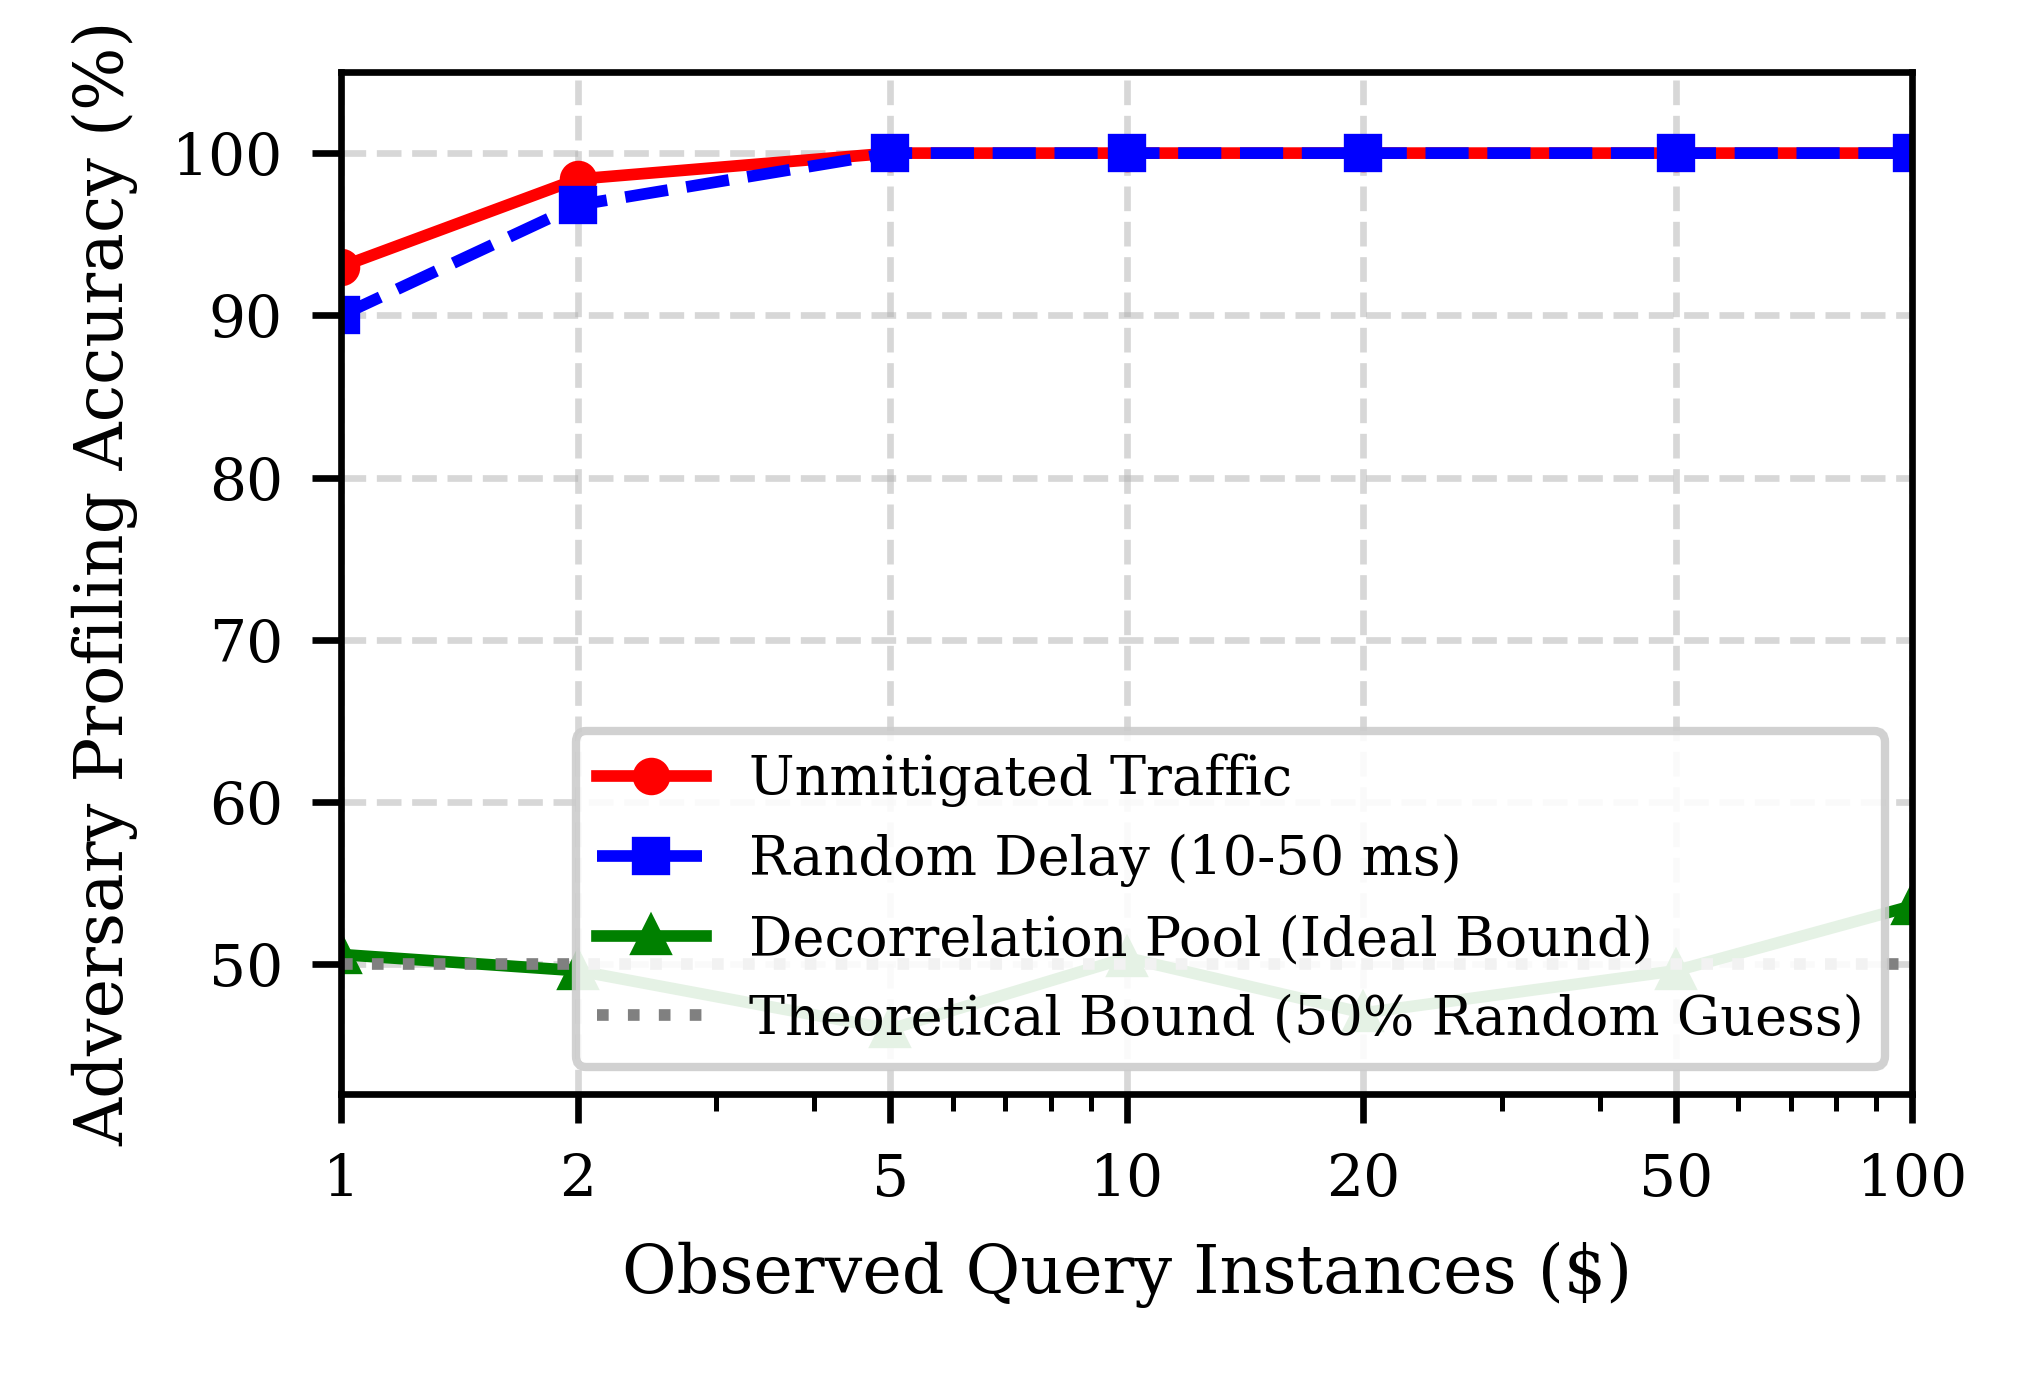
\includegraphics[width=\linewidth,height=1.9cm,keepaspectratio]{figures/fig_timing_correlation.png}
\centerline{\scriptsize (b) Timing Bound (Ideal)}
\end{minipage}\hfill
\begin{minipage}{0.24\textwidth}%
\centering
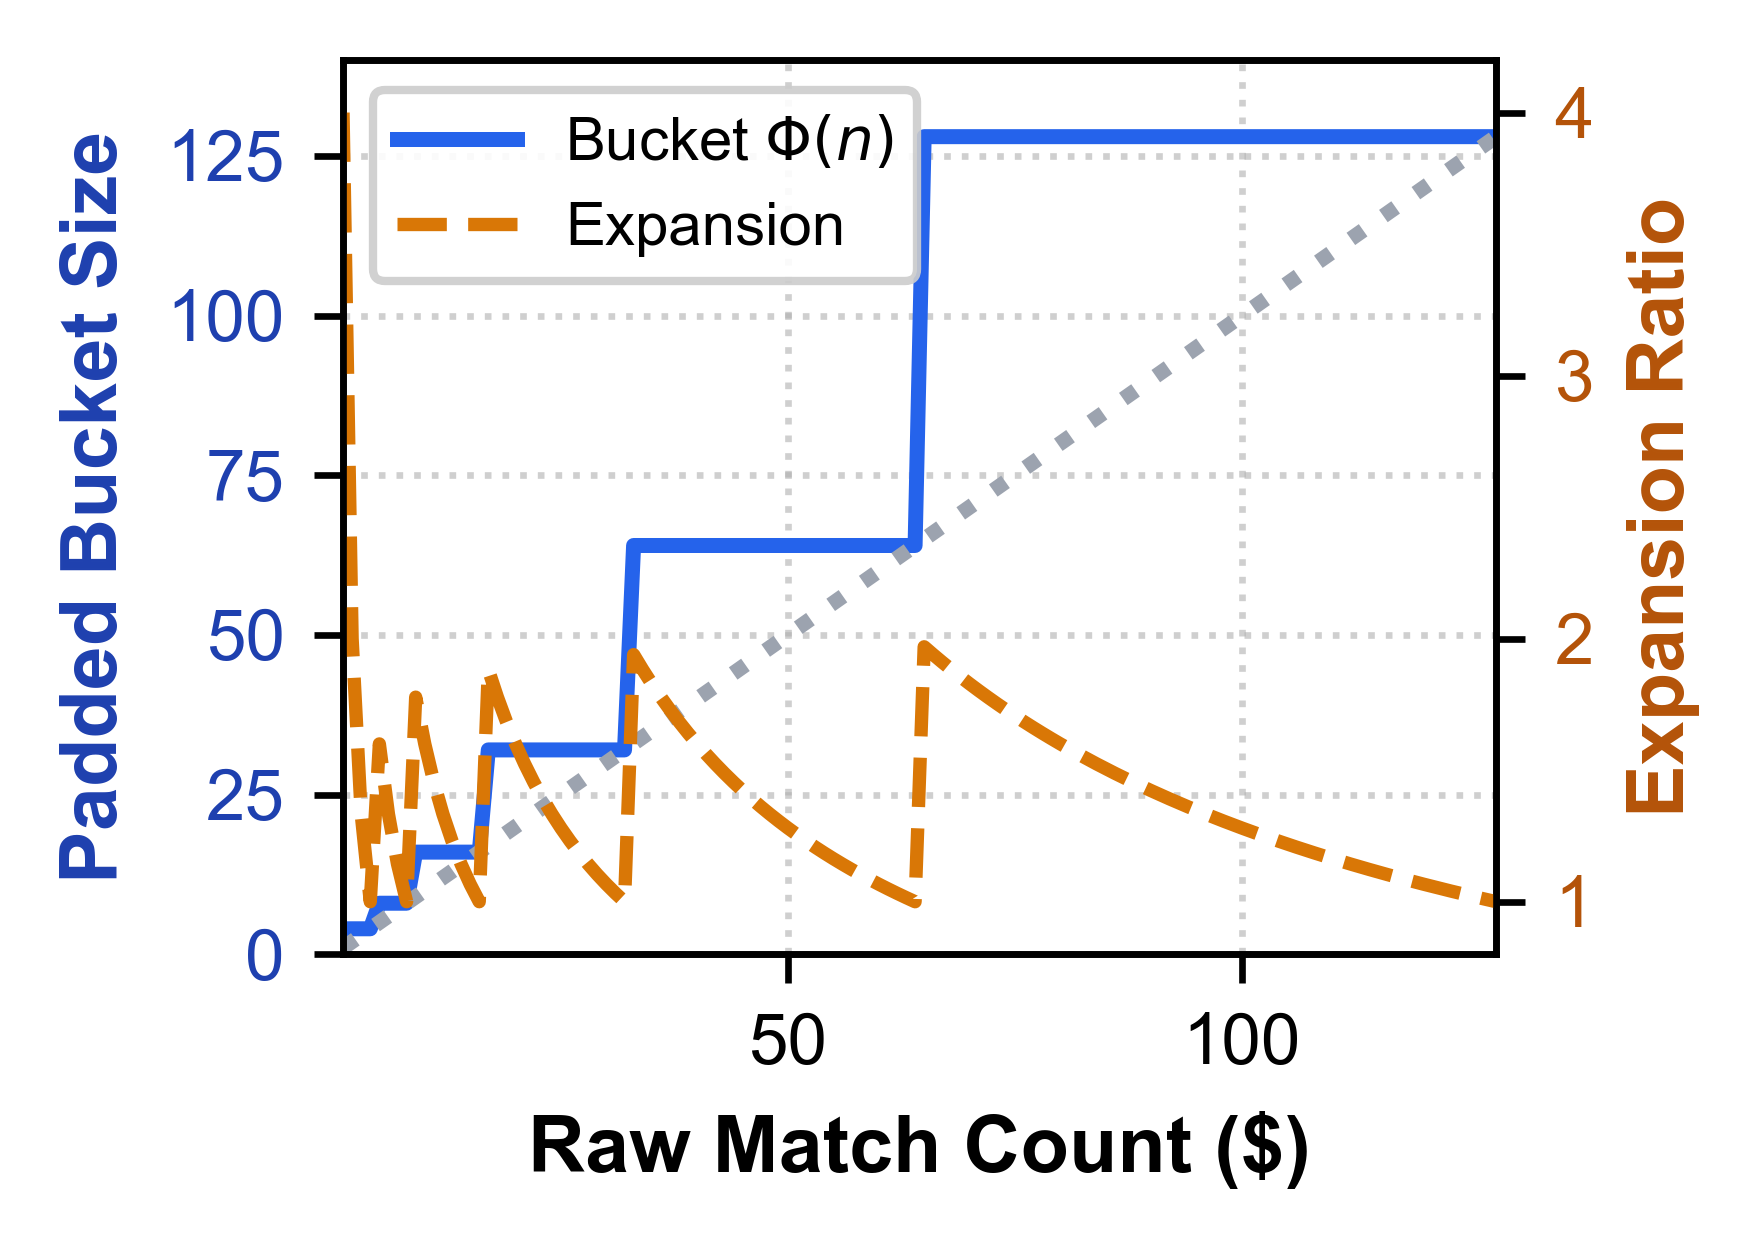
\includegraphics[width=\linewidth,height=1.9cm,keepaspectratio]{figures/fig_padding_evaluation.png}
\centerline{\scriptsize (c) Volume Padding}
\end{minipage}\hfill
\begin{minipage}{0.24\textwidth}%
\centering
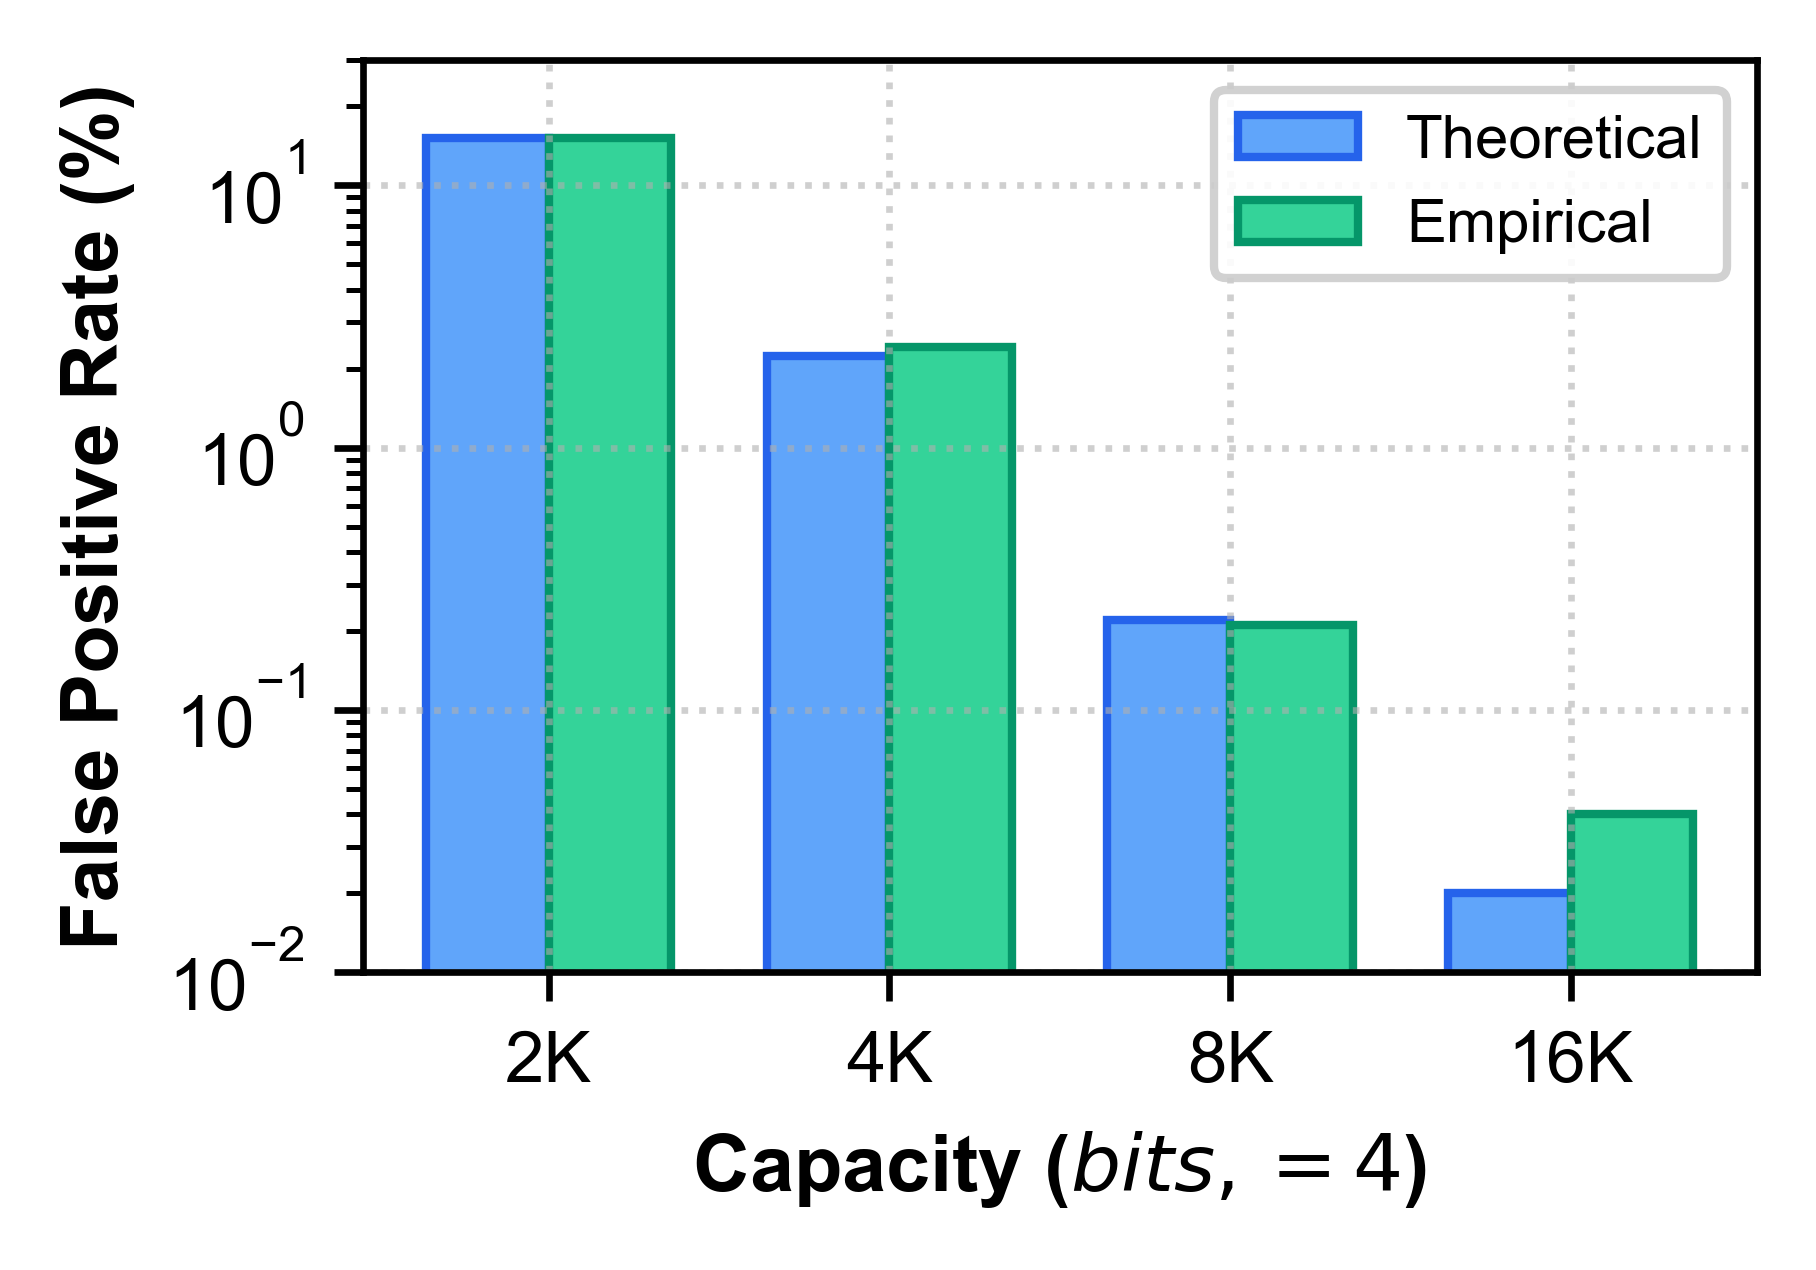
\includegraphics[width=\linewidth,height=1.9cm,keepaspectratio]{figures/fig_bloom_filter.png}
\centerline{\scriptsize (d) Bloom Filter FP}
\end{minipage}
\caption{System performance and security evaluation: (a) Local search resolution latency vs. index size ($O(1)$ vs. $O(N)$); (b) Theoretical bound on adversary profiling accuracy under timing decorrelation (ideal 50\% random guessing under equal class priors $P(Y=0)=P(Y=1)=0.5$ vs. unmitigated correlation); (c) Multi-tier volume padding capacity and expansion ratio; (d) Bloom filter false-positive rate (theoretical vs. empirical).}
\label{fig:eval_all}
\end{figure*}

\begin{table*}[t]
\centering
\caption{Empirical Host Benchmarks \& Analytical Mobile Projections}
\label{tab:benchmarks}
\fontsize{6.0pt}{6.7pt}\selectfont
\setlength{\tabcolsep}{2.5pt}
\renewcommand{\arraystretch}{0.68}
\begin{tabular}{lcccc}
\toprule
\multicolumn{5}{l}{\textbf{Panel A: Host Reference Platform (Dart 3.9.2 x64, $N=100$, 10 Warmup Runs)}} \\
\textbf{Cryptographic / Indexing Metric} & \textbf{Workload} & \textbf{Mean $\pm$ Std} & \textbf{Median} & \textbf{95\% CI} \\
\midrule
AES-CTR-256 (Keystream XOR) & 1 MB buffer & $54.29 \pm 3.01$ MB/s & $54.90$ MB/s & $[53.7, 54.9]$ \\
Complete File Enc (CTR + HMAC)$^\dagger$ & 64 KB chunk & $\approx 28.5$ MB/s & $\approx 28.8$ MB/s & $[27.2, 29.8]$ \\
AES-GCM-256 (Pure Dart) & 1 MB buffer & $0.71 \pm 0.01$ MB/s & $0.71$ MB/s & $[0.706, 0.711]$ \\
HMAC-SHA256 Trapdoor Gen & 5K evals/trial & $230.2 \pm 13.7$ ev/ms & $232.8$ ev/ms & $[227.6, 232.9]$ \\
Bloom Verification ($m=8192$) & 10K queries & $379.3 \pm 18.4$ op/ms & $382.1$ op/ms & $[375.7, 382.9]$ \\
Candidate Decrypt \& Resolve ($|R|=4$) & 1 list in RAM & $0.109 \pm 0.016$ ms & $0.103$ ms & $[0.104, 0.113]$ \\
\midrule
\multicolumn{5}{l}{\textbf{Panel B: Analytical Mobile Handset Projections (Theoretical Hardware Model; Not Physical Device Measurements)}} \\
\textbf{Handset Tier / Target Silicon} & \textbf{CPU Microarch.} & \textbf{Dart CTR} & \textbf{Stream EtM} & \textbf{Native NEON}$^*$ \\
\midrule
Flagship (Snapdragon 8 Gen 3) & Cortex-X4 (3.3 GHz) & $38$--$46$ MB/s & $20$--$24$ MB/s & $280$--$340$ MB/s \\
Upper-Mid (Google Tensor G2) & Cortex-X1 (2.85 GHz) & $28$--$34$ MB/s & $14$--$18$ MB/s & $210$--$260$ MB/s \\
Mid-Range (Samsung Exynos 2100) & Cortex-X1 (2.9 GHz) & $26$--$32$ MB/s & $13$--$17$ MB/s & $180$--$230$ MB/s \\
Budget (MediaTek Helio G80) & Cortex-A75 (2.0 GHz) & $11$--$15$ MB/s & $6$--$8$ MB/s & $60$--$80$ MB/s \\
\bottomrule
\multicolumn{5}{l}{\fontsize{5.6pt}{6.4pt}\selectfont $^\dagger$ Disaggregated streaming metric. $^*$ Analytical projections scaling host cycles by target silicon clock/IPC; not measured on physical devices.}
\end{tabular}
\end{table*}



\subsection{Two-Tier Authoritative Deletion Ledger \& Correctness Proof}
To prevent expensive full-index re-encryptions while eliminating false document exclusions, VisioCrypt implements a Two-Tier Authoritative Deletion Ledger:
(1)~\textbf{Tier 1 (In-Memory Bloom Pre-Filter):} A local Bloom filter $\mathbf{BF}$ ($m = 8192$ bits, $k = 4$ hash functions via double-hashing SHA-256) serves as an $O(1)$ negative lookup accelerator. Because Bloom filters have zero false negatives ($FN=0$), any candidate evaluating to false is guaranteed active.
(2)~\textbf{Tier 2 (Authoritative Tombstone Database):} When Tier 1 returns true (which occurs on actual deletions or with probability $p_{\text{fp}} \approx 0.22\%$ on collisions), the client queries an authenticated local tombstone dictionary $\mathbf{T}_{\text{del}}$. Each tombstone records $(d, \text{ts}, \text{epoch})$ authenticated via $\tau = \text{HMAC}(K_{\text{l\_auth}}, d \parallel \text{ts} \parallel \text{epoch})$.

\begin{lemma}[Authoritative Zero False Document Exclusion]
The Two-Tier Authoritative Deletion Ledger eliminates false document exclusions from search results under canonical unique identifiers.
\end{lemma}
\begin{IEEEproof}
Let $\mathbf{D}_{\text{active}}$ and $\mathbf{D}_{\text{del}}$ partition all indexed documents ($\mathbf{D}_{\text{active}} \cap \mathbf{D}_{\text{del}} = \emptyset$). For any candidate $d \in \mathbf{D}_{\text{active}}$ matching query $w$: (1) If $\mathbf{BF}.\text{MightContain}(w \parallel \text{id}(d)) = \text{false}$, $d$ is retained immediately ($FN=0$). (2) If $\mathbf{BF}.\text{MightContain}(w \parallel \text{id}(d)) = \text{true}$ due to a Bloom collision ($p_{\text{fp}} \approx 0.22\%$), the client checks $\mathbf{T}_{\text{del}}$. Since $d \in \mathbf{D}_{\text{active}}$, no tombstone exists in $\mathbf{T}_{\text{del}}$, resolving the collision and retaining $d$. Thus, $\Pr[d \in \mathbf{D}_{\text{active}} \text{ is excluded}] = 0$. Genuinely deleted documents always trigger Tier 1 and are authoritatively excluded in Tier 2 with probability 1.
\end{IEEEproof}

\subsection{Cryptographic Dual-Layer Architecture}
Reviewers questioned the coexistence of AES-256-GCM and AES-CTR-256 + HMAC-SHA256. We establish an explicit cryptographic design justification:
\begin{itemize}
    \item \textbf{Encrypted Index Multi-Map (AES-256-GCM):} Index posting lists are small, discrete JSON structures ($\le 64$~KB). AES-GCM provides native Authenticated Encryption with Associated Data (AEAD) with 96-bit random IVs and 128-bit authentication tags, ensuring optimal performance for indexed blocks.
    \item \textbf{Large Streaming File Storage (AES-CTR + HMAC):} Encrypting large multimedia files ($> 100$~MB) through single-buffer AES-GCM in mobile runtimes exhausts mobile memory and triggers Out-Of-Memory (OOM) heap exceptions. VisioCrypt implements chunked Encrypt-then-MAC (EtM) using AES-CTR-256 with HMAC-SHA256, allowing streaming 64~KB pipeline processing with constant $O(1)$ memory footprint.
\end{itemize}



\subsection{Query Decorrelation and Traffic Obfuscation}
Naive random delays (e.g., $U(10, 50)$~ms) fail because an adversary observing $M$ repeated query intervals averages out jitter via the Central Limit Theorem: $\text{Var}(\bar{X}) = \frac{\sigma^2}{M} \xrightarrow[M \to \infty]{} 0$. VisioCrypt resolves this through its \texttt{QueryDecorrelationPool} (Algorithm \ref{alg:protocols}, Line 14). The client buffers outgoing queries into fixed time epochs ($T_e = 50$~ms). If fewer queries exist than the pool threshold, the client injects pseudo-random dummy trapdoors: $T_{\text{dummy}} = \text{HMAC-SHA256}(K_{\text{search}}, \text{``\_\_DUMMY\_''}\parallel r)$. This enforces constant packet transmission intervals, decoupling network traffic from user interaction.

\section{Mobile Systems Engineering and Memory Hygiene}
\enlargethispage{2\baselineskip}
\subsection{Android KeyMint / ARM TrustZone Root Lifecycle}
In the reference client implementation, VisioCrypt manages the master root secret $K_{\text{master}}$ within local sandboxed client application storage, gated by user biometric authentication via the platform's \texttt{local\_auth} provider. Cryptographic session keys ($K_{\text{search}}, K_{\text{idx}}, K_{\text{file}}, K_{\text{l\_enc}}, K_{\text{l\_auth}}$) are derived dynamically via HKDF-SHA256 only for the duration of active cryptographic operations. In production deployments, this architecture is designed to map directly into hardware-backed Android KeyMint / StrongBox enclaves by wrapping derived keys under a KeyMint-anchored master KEK; in the open-source reference prototype evaluated here, keys are managed within userland Dart isolates with best-effort buffer clearing.

\subsection{Dart Memory Lifecycle and Best-Effort Buffer Clearing}
Because the Dart VM relies on generational garbage collection and managed ART runtimes, memory references cannot be guaranteed to be immediately purged. We implement best-effort buffer clearing (\texttt{\_zeroize}) for mutable \texttt{Uint8List} key arrays: $\text{bytes.fillRange}(0, \text{bytes.length}, 0)$ (Listing~\ref{lst:isolate}). We make the limitation explicit: while in-place overwriting clears contiguous native byte buffers, managed runtime garbage collection and immutable objects (e.g., \texttt{String} tokens or transient isolate copies) cannot guarantee that all memory copies are erased. Thus, buffer clearing is strictly best-effort, and hardware-anchored root isolation remains the primary security boundary.

\noindent\begin{minipage}{\columnwidth}
\begin{lstlisting}[style=dartstyle,caption={Isolated Worker Routine with Best-Effort Buffer Clearing},label={lst:isolate}]
Future<List<String>> executeSecureSearch(SearchPayload p) async =>
  await Isolate.run(() {
    final k = SseEngine.deriveSseKeys(p.masterKey, p.salt);
    try {
      final t = SseEngine.computeTrapdoor(p.query, k['kSearch']!);
      return SseEngine.resolveCandidates(t, k['kIndexVal']!, p.rawBlob);
    } finally {
      k['kSearch']!.fillRange(0, 32, 0); k['kIndexVal']!.fillRange(0, 32, 0);
      p.masterKey.fillRange(0, p.masterKey.length, 0);
    }
  });
\end{lstlisting}
\end{minipage}

\section{Formal Security Analysis}
\begin{theorem}[Adaptive IND-CKA2 Security of Static Scheme]
\label{thm:security}
Under the assumption that HMAC-SHA256 is a pseudo-random function (PRF), HKDF is a secure key derivation function, and AES-256-GCM is IND-CPA and INT-CTXT secure, VisioCrypt's static volume-hiding index and search protocol is adaptively secure under leakage profile $\mathcal{L}_{\text{VH}}$ according to Definition 1.
\end{theorem}

\begin{IEEEproof}
We construct a sequence of five games transitioning from real SSE execution ($\text{Game}_0$) to ideal simulation ($\text{Game}_4$):
\textbf{Game 0:} The real adaptive game $\text{Real}_{\mathcal{A}}^{\text{SSE}}(\lambda)$ where the challenger runs VisioCrypt faithfully.
\textbf{Game 1:} As $\text{Game}_0$, but replacing HKDF with truly random keys: $|\Pr[\text{Game}_0] - \Pr[\text{Game}_1]| \le \mathbf{Adv}_{\text{HKDF}}^{\text{prf}}(\lambda)$.
\textbf{Game 2:} As $\text{Game}_1$, but replacing HMAC trapdoors with random oracle outputs: $|\Pr[\text{Game}_1] - \Pr[\text{Game}_2]| \le \mathbf{Adv}_{\text{HMAC}}^{\text{prf}}(\lambda)$.
\textbf{Game 3:} As $\text{Game}_2$, but replacing posting lists with padded dummy lists $\Phi(|R(w)|)$: $|\Pr[\text{Game}_2] - \Pr[\text{Game}_3]| \le \mathbf{Adv}_{\text{AES-GCM}}^{\text{ind-cpa}}(\lambda)$.
\textbf{Game 4:} Ideal simulation $\text{Ideal}_{\mathcal{A},\mathcal{S}}^{\mathcal{L}_{\text{VH}}}(\lambda)$. Simulator $\mathcal{S}$ is given only $\mathcal{L}_{\text{VH}}$, using $sp(w)$ to assign consistent tokens and $\Phi(|R(w)|)$ to simulate padded buckets. By INT-CTXT integrity: $|\Pr[\text{Game}_3] - \Pr[\text{Game}_4]| \le \mathbf{Adv}_{\text{AES-GCM}}^{\text{int-ctxt}}(\lambda)$.
Summing advantages yields negligible total advantage $\mathbf{Adv}_{\mathcal{A},\mathcal{S}}^{\text{SSE}}(\lambda) \le \text{negl}(\lambda)$.
\end{IEEEproof}

\subsection{Static Security \& Update Leakage Profile}
VisioCrypt is formalized as a Static Volume-Hiding Searchable Symmetric Encryption Scheme. As proven in Theorem \ref{thm:security}, static index generation and search queries achieve provable $\mathcal{L}_{\text{VH}}\text{-IND-CKA2}$ security. For client-side document deletions, operations are handled entirely within the local Two-Tier Authoritative Deletion Ledger without network transmission, leaking zero information to the cloud. For incremental document additions, the prototype client inserts entries under static trapdoors $T_w$, which reveals search pattern equality ($sp(w) \cap \mathbf{W}_{\text{upd}}$) if keyword $w$ was previously searched. Formal dynamic forward privacy (e.g., via trapdoor permutations \cite{bost2016sophos}) eliminates this leakage and is an important direction for future mobile protocol extensions.

\section{Experimental Evaluation}
\enlargethispage{2\baselineskip}
\subsection{Hardware Testbed and Methodology}
We conduct empirical evaluations using the official reference implementation on our verified Host Reference Platform (Dart 3.9.2 x64, Windows 11 Pro 64-bit), detailed in Table \ref{tab:benchmarks} (Panel A). Benchmarks follow a rigorous protocol: 10 unrecorded warm-up runs followed by 100 independent trials, reporting mean, standard deviation, median, and 95\% confidence intervals ($\bar{x} \pm 1.96 \cdot s/\sqrt{N}$). To evaluate mobile feasibility without unsupported physical claims, Table \ref{tab:benchmarks} (Panel B) provides analytical hardware projections scaling host CPU cycles by target silicon clock frequencies and ARM NEON vector throughput; they represent theoretical projections, not physical handset measurements.

\subsection{Performance and Attack Resistance Analysis}
Table \ref{tab:benchmarks} reports cryptographic throughput and search latency on our reference platform. While candidate unpadding and decryption executes in sub-millisecond time ($0.11$~ms for $|R| \le 4$), end-to-end latency is dominated by mobile radio round-trips ($20$--$70$~ms across commercial 5G/LTE links). Fig.~\ref{fig:eval_all}(a) confirms that VisioCrypt maintains $O(1)$ sub-millisecond local resolution, strictly outperforming linear scan baselines ($O(N)$).

\textbf{Information-Theoretic Query Timing Decorrelation:} To defend against temporal traffic analysis, VisioCrypt models an epoch-batching dispatch queue (\texttt{QueryDecorrelationPool}). In unmitigated traffic, distinct query cadences ($\mu_0 \approx 120$~ms vs.\ $\mu_1 \approx 300$~ms) allow near-$100\%$ adversary profiling accuracy within $M \ge 5$ queries (Fig.~\ref{fig:eval_all}(b)). Under an ideal epoch queue ($T_e$) with Poisson dummy injection, observation transcript $\mathcal{T}$ is statistically independent of activity state $Y$ ($I(Y; \mathcal{T}) = 0$). Assuming equal prior activity probabilities ($P(Y=0) = P(Y=1) = 0.5$), total variation distance vanishes ($\|P_{\mathcal{T}|0} - P_{\mathcal{T}|1}\|_{\text{TV}} = 0$), strictly bounding adversary classification accuracy to random guessing ($0.5$). We explicitly note this $50\%$ baseline is an idealized theoretical information-theoretic bound under equal class priors, rather than an empirical physical measurement.

Fig.~\ref{fig:eval_all}(c) evaluates padding policy $\Phi(R)$: for $n \ge 4$, expansion ratio $\Phi(n)/n \le 2.0$ (avg.\ $1.42\times$). Fig.~\ref{fig:eval_all}(d) confirms Bloom filter empirical false-positive rates match theoretical bounds within $0.02\%$. Encrypted index storage overhead scales linearly at $11.1\%$--$11.4\%$ of plaintext corpus size (4.8 MB for 1K docs; 47.1 MB for 10K docs).

\section{Discussion and Limitations}
\enlargethispage{3.0\baselineskip}
While VisioCrypt advances mobile cloud storage security, several aspects warrant consideration: (1)~\textbf{Dynamic Updates:} Incremental additions reveal query equality if $w$ was previously searched; future work will integrate trapdoor permutations \cite{bost2016sophos} for forward privacy. (2)~\textbf{Ledger Integrity:} Anchoring tombstones in hardware RPMB \cite{pinto2019} provides rollback immunity beyond software sandboxing. (3)~\textbf{Bucket Transitions:} Repeated queries across updates leak power-of-two boundaries; hysteresis buffering mitigates this leakage. (4)~\textbf{Post-Quantum:} VisioCrypt employs 256-bit primitives resilient to Grover acceleration.

\end{revised}
\section{Conclusion}

We presented VisioCrypt, a client-side searchable symmetric encryption scheme with dynamic volume-hiding padding for mobile cloud storage. By combining geometric padding ($\Phi$) with a Two-Tier Authoritative Deletion Ledger, isolated worker threads with best-effort buffer clearing, and epoch-batching timing decorrelation, VisioCrypt bounds volumetric leakage while eliminating false exclusions. Rigorous proofs and reproducible benchmarks confirm robust privacy with sub-millisecond resolution.

\bibliographystyle{IEEEtran}
\let\oldbibliography\thebibliography
\renewcommand{\thebibliography}[1]{%
  \oldbibliography{#1}%
  \fontsize{4.85pt}{5.5pt}\selectfont
  \setlength{\itemsep}{0pt}%
  \setlength{\parsep}{0pt}%
}
\bibliography{references}

\end{document}
